The Single Instruction Multiple Data (SIMD) architecture was popular in the
1990s.
%
With SIMD architecture, all processing elements (PE) execute identical instructions
cycle by cycle, but they access different local data from their private 
local memory.
%
All PEs are also connected in a net structure, allowing
communication between them.
%
Figure~\ref{fig:simd1} illustrates an example SIMD architecture.

\begin{figure}
    \centering
    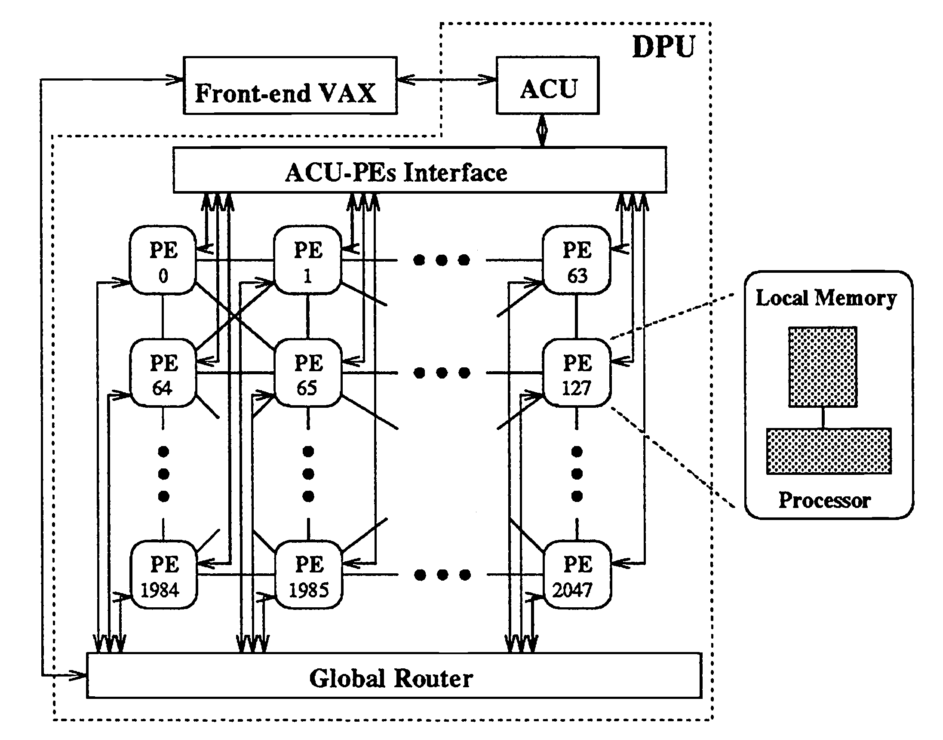
\includegraphics[width=0.8\textwidth]{fig/simd.png}
    \caption{An example of the SIMD architecture: the MasPar system.}
    \label{fig:simd1}
\end{figure}


Lee et. al. implemented DWT on a SIMD machine, the MasPar
system~\cite{lee1994parallel}.
%
MasPar has 2048 PEs organized in a 64x32
mesh topology, as shown in Figure~\ref{fig:simd1}.
%
This implementation takes use of the row structures of available PEs,
by mapping an one-dimensional input signal onto a row of PEs to process.
%
More specifically, a row of PEs take input values and performe calculations 
together, and passes the output coefficients to the next row of PEs.
%
The next row of PEs then performs the next iteration of DWT on the input
coefficients.
%
At the same time, the first row of PEs takes in new input to calculate on.
%
This process is illustrated in Figure~\ref{fig:simd2}.


\begin{figure}
    \centering
    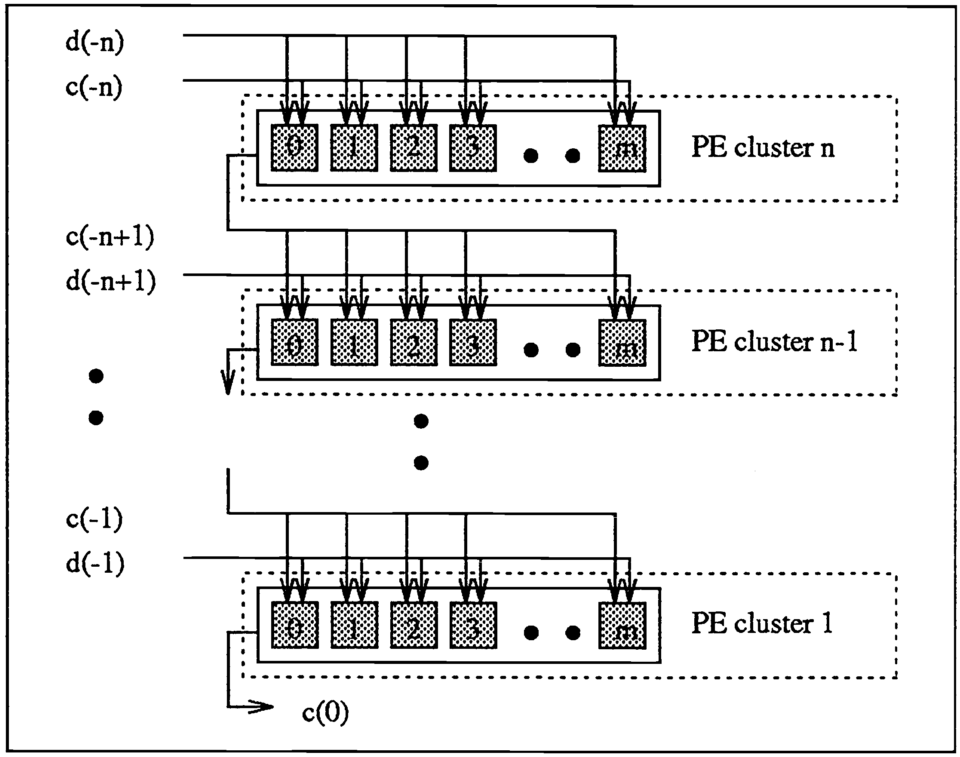
\includegraphics[width=0.8\textwidth]{fig/simd2.png}
    \caption{The pipeline of rows of PEs executing same instructions.
             The output of previous row serves as input for the next row
             of PEs to perform the next iteration of DWT.}
    \label{fig:simd2}
\end{figure}


From the perspective of parallel execution, this implementation uses
a pipeline pattern to achieve great parallelism.
%
As we discussed in class, the amount of parallelism achieved depends on
the number of iterations of DWT we could perform on the input signal.
%
This implementation might not be able to make use of all PEs if run on 
a very large system with many rows of PEs.


The experiment shows that the parallel implementation has a better 
performance than that of a serial implementation on the SPARC 1 workstation,
whose processor is at least 100 times faster than that of the MasPar.
%
Scalability wise, this pipeline implementation is able to keep good speedups
when the problem size grows.
%
This is because larger problems naturally enable more iterations of DWT
to apply on.
%
As a result, the execution pipeline has more steps, and can run more efficiently.
